\subsection{Shielding}

\subsubsection{Incident, reflected and transmitted waves in medium}

In the following, the fundamental theory of electromagnetic shielding is presented. A figure of merit for shielding capabilities of a material is the electromagnetic shielding effectiveness $SE$, given in \cites{10518640}[p. 63]{Jaroszewski_Thomas_Rane_2019}

\begin{equation}
	SE_{\mathrm{dB}}=20\log{\left(\frac{E_\mathrm{i}}{E_\mathrm{t}}\right)}.
	\label{eqn:se_elec_fields}
\end{equation}

$E_\mathrm{i}$ denotes the incident electric field intensity, while $E_\mathrm{t}$ represents the transmitted electric field intensity, as illustrated in \autoref{fig:shielding_material_diagram}. These values depend on the material’s thickness, geometry, and its electric and magnetic properties.

\begin{figure}[h]
    \centering
    \includegraphics[width=0.35\linewidth]{content/img/shielding_material_diagram.png}
    \caption{Incident, reflected and transmitted electric field intensities at a shielding material.}
    \label{fig:shielding_material_diagram}
\end{figure}

% (Note: Higher order modes may be able to propagate in the TEM cell, as the refraction of the shielding material follows to excitation of these modes.)

An electromagnetic wave can undergo reflection, absorption or multiple reflections within the shielding material, with each reflection contributing to the total reflected, absorbed, and transmitted wave. The main contribution of a material's shielding effectiveness is reflection \cite[p. 1]{Jaroszewski_Thomas_Rane_2019}. The total shielding effectiveness is determined by \cite[p. 63]{Jaroszewski_Thomas_Rane_2019}

\begin{equation}
	SE_{\mathrm{dB}}=R_{\mathrm{dB}}+A_{\mathrm{dB}}+B_{\mathrm{dB}},
	\label{eqn:se_rereflections}
\end{equation}

according to Schelkunoff's approach to shielding \cite{Schelkunoff_1938}. Absorption losses $A_{\mathrm{dB}}$ arise from waves propagating through the shield, $R_{\mathrm{dB}}$ denotes reflections at the material's surface, and $B_{\mathrm{dB}}$ is a correction factor accounting for multiple reflections within the shield \cite{10518640}. However, when investigating shielding materials with thicknesses less than the skin depth, $B_{\mathrm{dB}}$ can be neglected \cite[p. 1]{Jaroszewski_Thomas_Rane_2019}. While absorption $A_{\mathrm{dB}}$ is related to the skin depth, the thinness of the shielding material shifts the emphasis to reflection as the primary shielding mechanism. The concept of skin depth is still discussed in \cref{sec:skin_effect}.

Reflections are caused by wave impedance mismatch between to materials, and are characterized by the reflection coefficient $R$. It is common practice to normalize the wave impedance $Z$ to the free-space wave impedance $Z_0$. At the interface between free space and a shielding material, this yields \cite{Collin_2015}

\begin{equation}
	R=\frac{Z-1}{Z+1}.
	\label{eqn:reflection_coefficient_plane_dielectric}
\end{equation}


\subsubsection{Electrical characteristics}

The normalized wave impedance is given by

\begin{equation}
    Z=\frac{1}{Z_0}\sqrt{\frac{\mathrm{i}\omega\mu}{\sigma+\mathrm{i}\omega\epsilon}}.
    \label{eqn:rel_wave_imp}
\end{equation}



%The reflection coefficient can be converted into dB, leading to $R_\mathrm{dB}$. Any additional reflection happen due to re-reflections inside the shielding material, described by $B_\mathrm{dB}$. The rest of the energy must either be absorbed, described by $A_\mathrm{dB}$ or transmitted, shown by $T_\mathrm{dB}$. 

%\todo{p. 309 Classical Electrodynamics (John David Jackson) describe shielding material by dipole moments}


%The wavenumber $k$ in lossy media consists of a real and an imaginary, parts as in
%
%\begin{equation}
%	k = \beta + \mathrm{i}\alpha.
%	\label{eqn:wave_number}
%\end{equation}

%The imaginary part of the wavenumber $k$, $\alpha$ denotes the attenuation or absorption coefficient. It describes the reduction of the intensity of the wave over distance.

When molecules in a material are exposed to an electric field, they become polarized. This property is characterized by the material's permittivity $\epsilon$. Exposure to a magnetic field causes the spins of electrons within atoms to align with the field, described by the material’s permeability $\mu$. When these electric and magnetic fields vary with time, the molecules continuously move and realign, resulting in the movement of charges, which is quantified by the conductivity $\sigma$. The energy lost in this dynamic process is dissipated as heat \cite{Balanis_2012}.

The electric field will push charges in polarizable molecules apart. This separation of charges may be described as a electric dipole, depending on the separation distance and the charge. Under alternating electric fields, the moving of charges will contribute to $\sigma$. This phenomenon is called dielectric hysteresis. It is quantified by the loss tangent $\tan\delta_e$, and defined as \cite{Balanis_2012}

\begin{equation}
	\tan\delta_e = \frac{\sigma_s}{\omega\epsilon'}+\frac{\epsilon''}{\epsilon'}.
	\label{eqn:loss_tangent_permittivity}
\end{equation}

There, $\sigma_s$ is the static conductivity, indicating the conductivity of the material for constant fields over time. The complex part of the permittivity $\epsilon''$ describes the lossy part of the dielectric material, specifically relevant for alternating fields over time. The real part of the permittivity is lossless and is noted by $\epsilon'$, and corresponds to the material's ability to store electric energy \cite{Kruželák_Kvasničáková_Džuganová_Dosoudil_Hudec_Krump_2024}. The overall complex permittivity is therefore $\epsilon=\epsilon'+\mathrm{i}\epsilon''$.

The loss tangent relates therefore the conductivity of a material to the real permittivity. A dielectric with low losses has a much larger displacement current than conduction current density ($\tan\delta_e \ll 1$). The opposite is true for a good conductor ($\tan\delta_e \gg 1$) \cite{Balanis_2012}.

%The loss tangent $\tan\delta_e$ is a function of frequency, however, it is often not stated as such. Therefore, the loss tangent of FR4, for example, is given as $\tan\delta_e=0.02$ for frequencies up to 1\,GHz. For higher frequencies, the molecules may have resonance frequencies, where they influence more strongly the overall conductance and consequently increase the imaginary part of the permittivity $\epsilon''$.

Analogous to polarizable material, there are also magnetizable lossy materials, which is characterized by a complex permeability $\mu=\mu'+\mathrm{i}\mu''$. The real part of the permeability $\mu'$ described the material's ability to store magnetic energy, while $\mu''$ described the magnetic losses  \cite{Kruželák_Kvasničáková_Džuganová_Dosoudil_Hudec_Krump_2024}. The complex permeability can also be described by a magnetic loss tangent $\tan{\delta_m}$, as shown in

\begin{equation}
	\tan{\delta_m}=\frac{\mu''}{\mu'}.
	\label{eqn:magnetic_loss_tangent}
\end{equation}

Although, the loss tangent is very low for the majority of materials and will be neglected. Ferrites are an exception, which are commonly used to dampen high frequency signals \cite{Balanis_2012}.

Electric fields dominate in the near-field region of electric dipoles, as discussed in \cref{sec:ele_dip}. Consequently, the wave impedance in this region is very high. For effective shielding by reflection, the shielding material should possess high permittivity and high conductivity to achieve a low impedance (see \autoref{eqn:rel_wave_imp}), creating the necessary impedance mismatch for reflection \cite[p. 67]{Jaroszewski_Thomas_Rane_2019}.

In contrast, magnetic fields are predominant in the near-field region of magnetic dipoles, as demonstrated with \cref{sec:mag_dip}. A high conductivity shields well against high-frequency magnetic fields due to creation of counter-acting eddy currents \cite[p. 112]{Jaroszewski_Thomas_Rane_2019}. Low-frequency magnetic fields are difficult to shield, and the most common approach is the redirection of magentic flux line due to high permeability of the shielding material \cite[pp. 112-113]{Jaroszewski_Thomas_Rane_2019}.

\subsubsection{ASTM ES7-83 Method}\label{sec:astm}

The ASTM ES7-83 method is used to determine the shielding effectiveness of shielding materials. The shielding material is inserted into a coaxial TEM cell around the septum. Ideally, they form a continuous connection \cite{MORARI_BĂLAN_2015}. 

In this method, two measurements are performed with an oscilloscope attached to the output of the TEM cell. In the first, an empty TEM cell is excited and a reference output voltage $U_\mathrm{ref}$ is measured. In the second, the TEM cell is loaded with the shielding material, and the output voltage $U_\mathrm{load}$ is again noted. The measurement values are then used in 

\begin{equation}
	SE_\mathrm{dB}=20\cdot\log{\left(\frac{U_\mathrm{ref}}{U_\mathrm{load}}\right)}.
	\label{eqn:SE_voltages}
\end{equation}

to derive the shielding effectiveness $SE_\mathrm{dB}$ \cite{MORARI_BĂLAN_2015}.

When applying numerical analysis in combination with this method, it is more convenient to defined a reference output power $P_\mathrm{ref}$ for an unloaded TEM cell, and an output power for the loaded case $P_\mathrm{load}$. This leads to the similar 

\begin{equation}
	SE_\mathrm{dB}=10\cdot\log{\left( \frac{P_\mathrm{ref}}{P_\mathrm{load}} \right)}.
	\label{eqn:SE_power}
\end{equation}

Additionally, a rectangular TEM cell is used for this method, instead of the commonly used cylindrical version. \autoref{fig:form_of_shielding_material} shows the cross section of this shielding material, which is inserted into the TEM cell. In \autoref{fig:ASTM ES7-83} the shielding material can be seen wrapped around the septum. 

\begin{figure}[h]
    \centering
    \begin{subfigure}[h]{0.49\textwidth}
        \centering
        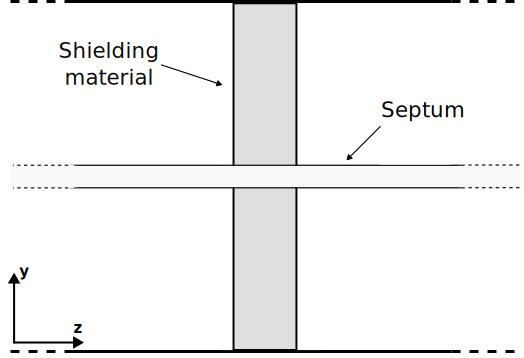
\includegraphics[width=\textwidth]{content/img/ASTM ES7-83.png}
        \caption{Shielding material in TEM cell}
        \label{fig:ASTM ES7-83}
    \end{subfigure}%
    \hfill
    \begin{subfigure}[h]{0.49\textwidth}
        \centering
        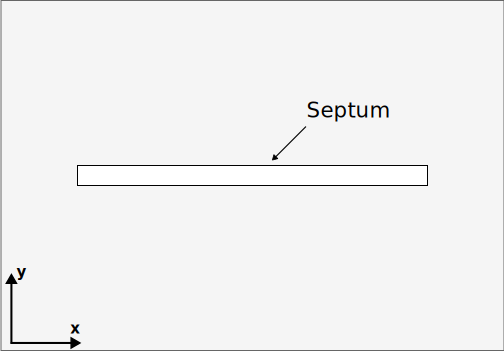
\includegraphics[width=\textwidth]{content/img/form_of_shielding_material.png}
        \caption{Shape of the shielding material}
        \label{fig:form_of_shielding_material}
    \end{subfigure}
    \label{fig:subfigures}
\end{figure}

Then, the S-parameters derived in the simulations are used to get to the output powers $P_\mathrm{ref}$ and $P_\mathrm{load}$. By exciting the TEM cell with a power of 1\,W, the reference power $P_\mathrm{ref}=1\,\mathrm{W}$. The measured power is then derived through

\begin{equation}
    P_\mathrm{load}=P_\mathrm{ref}\cdot10^{|S_\mathrm{12, dB}|/10}.
    \label{eqn:load_power}
\end{equation}

\subsubsection{Dual TEM cell}\label{sec:dual_tem_cell}

The shielding effectiveness of a material may also be determined using a dual TEM cell shown in \autoref{fig:dual_tem_cell}. They are connected through an aperture, which can be filled with the shielding material or left empty. The upper TEM cell is excited through port 1, and acts as a driving cell, transmitting power through the aperture. Port 2 is loaded with the reference impedance $Z_w\approx50\,\Omega$. The second TEM cell functions as a receiver, collecting power at its output ports \cite{MORARI_BĂLAN_2015}.

\begin{figure}[h]
	\centering
	\includegraphics[width=0.75\linewidth]{content/img/dual_tem_cell.png}
	\caption{Dual TEM cell with aperture}
	\label{fig:dual_tem_cell}
\end{figure}

If the aperture is electrically small, its coupling may be described by an electric and a magnetic dipole moment. Their magnitude is related to the electric and magnetic coupling between the TEM cells over the aperture. Therefore, the electric and magnetic coupling can be determined separately by adding or subtracting the output powers of the receiving TEM cell \cite{MORARI_BĂLAN_2015, 4091811}. Consequently, a electric shielding effectiveness $SE_\mathrm{dB}^\mathrm{e}$ and a magnetic shielding effectiveness $SE_\mathrm{dB}^\mathrm{m}$ can be calculated with

\begin{subequations}
	\begin{equation}
		SE_\mathrm{dB}^\mathrm{e}=10\log{\left( \frac{P_\mathrm{ref, sum}}{P_\mathrm{load,sum}} \right)},
		\label{eqn:se_dual_cell_e}
	\end{equation}
	\begin{equation}
		SE_\mathrm{dB}^\mathrm{m}=10\log{\left( \frac{P_\mathrm{ref, diff}}{P_\mathrm{load,diff}} \right)}.
		\label{eqn:se_dual_cell_m}
	\end{equation}
\end{subequations}

Separating the electric and magnetic shielding effectiveness is useful when applying shielding materials in the near field of electric or magnetic dipole moments. For shielding a magnetic dipole moment, the $SE_\mathrm{dB}^\mathrm{m}$ value is considered significant \cite{4091811}, whereas for an electric dipole moment, the $SE_\mathrm{dB}^\mathrm{e}$ value is relevant.

%Because the normalized electric field at the aperture will be of TEM mode, only the component normal to the aperture in z-direction has to be considered. Just as in the case of dipole representation, the Lorentz Reciprocity theorem may be applied to find the fields in the TEM cell. Because both the fields at the output and in the aperture are of TEM mode, only the E-field at the output may be considered. 



